\documentclass[11pt, a4paper, notitlepage]{report}
\usepackage[utf8]{inputenc} % Ensures we can use UTF8.
\usepackage[round,colon]{natbib}
\bibliographystyle{hull}
\usepackage{amsmath}
\usepackage{graphicx}
\graphicspath{ {./images} }
\usepackage{hyperref} % Must come last; allows for links.
\hypersetup{
    hidelinks
}

\title{Smart Kart}
\date{April 2022}
\author{George Jacob Anthony Kokinis}
\begin{document}
\maketitle
\begin{center}
    Student Number 201910280
    
    Word Count: ?? %exclude acknowledgements, abstract, table of contents, references and appendices) of your document.
\end{center}
\newpage
\section{Abstract}
Average speed check zones (ASC zones), typically enforced using SPECS\footnote{SPECS \citep{specsjenop}} in the UK, are being increasingly deployed in throughout the UK; doubling between 2013 and 2016 \citep{BBCSpeedCameraDoubled}. While useful for enforcing speed limits and increasing safety, with \citet{owenAllsop} finding that fatal and serious collisions dropped by 36.4\% at ASC zones installed purposely to reduce collisions, ASC Zones can lead to distracted driving, as the driver has to monitor their speed, which means looking away from the road to their speedometer for brief periods of time.

This project seeks to create a software application for a smartphone, that detects when a vehicle the phone is in enters an ASC zone, starts tracking the vehicle's speed, and gives the driver an audible alert if their average speed is at risk of breaking the speed limit, so as to reduce dependence on the driver to check their speedometer.

\tableofcontents

\chapter{Introduction}
\section{Context}\label{sec:Context}
Average speed check zones are an alternative to traditional fixed point speed cameras. Fixed point cameras take two photos a given time-delta apart and measure the car's distance using road markings, to calculate the speed: $ speed = distance \div time $. This is good for enforcing speed in that one position, but does no enforcement for the road before or after the camera. In contrast, ASC zones effectively use the same methodology but across a longer distance (such as half a mile or 1.5 miles between cameras, and a series of cameras across tens of miles); hence effectively enforcing the speed limit across much larger areas of road.

Currently, there are various products for monitoring a driver's speed and for indicating speed cameras; the main smartphone applications in this space are Google Maps \citep{googleMaps} and Waze \citep{waze}; while Apple Maps \citep{appleMaps} will inform you of fixed speed cameras\footnote{In the UK, these were originally "Gatso" cameras, later followed by Truvelo and Truvelo d-cam \citep{dcam}}, it does not inform you of ASC zones.

However, Google Maps does not register ASCs as actual "zones", but instead as a fixed speed camera at the start of the zone. Waze displays your progression through an ASC, but does not calculate your average speed. TomTom GO Navigation \citep{tomtomGo} does track your average speed in an ASC zone, but operates on a paid subscription model, so is not available to everyone. Hence, there is space in the market for a free solution to monitoring speed in ASC zones.
\section{The Problem}
While lawful drivers should be aware of their speed anyway, it is likely that many check their speed more often and with more discretion whilst within an ASC zone. This means they may be focused on their speedometer when something important is passed, such as a direction sign, a signal from another road user, or an overhead gantry message - such as the "Red X" on Smart Motorways\footnote{Smart Motorways \citep{SmartMotorways}}, or a speed limit change. 
\section{A solution}
By creating a smartphone application that warns a user if they are about to 
exceed the speed limit, the load on the driver can be reduced, allowing them to 
have more awareness of the road. By making this application free to use 
(whether free or supported by advertisements), this increases availability, 
potentially increasing the impact of this project.
\section{Report Structure}
The rest of this report is structured into the following chapters:
\begin{itemize}
	\item Background: Describing and laying out technologies and concepts that may be used in the development of the application or are useful for understanding other technologies.
	\item Aims and Objectives: Specification in detail about what features the application should have and how this will be tested or measured.
	\item Design: A description of the initial design, visual and technical, for the application, and design(s) for surveys to gain feedback on the UI of the application.
	\item Technical Development: Discussion around the development of the application. Note that the actual development log will be listed in Appendix \ref{app:GitLog}.
    \item Evaluation: Discussion and Evaluation of how closely the application meets the Aims and Objectives in the aforementioned chapter.
\end{itemize}
After which there will be Appendices and the Bibliography. % Remove this?
\chapter{Background}
The development of this project requires understanding and examination of various topics across various fields; including Kinematics, Programming, Law, and UX. Hence this chapter discusses and describes relevant topics.
\section{Speed Cameras}
\subsection{Fixed-Point Cameras}
In the United Kingdom, traditional fixed-point speed cameras were of a "Gatso" type, later replaced by "Truvelo", and later Truvelo D-Cam. They are installed either by the Local Authority, the local Police Force, or the relevant highways agency\footnote{\textit{National Highways} in England, \textit{Transport Scotland} in Scotland, \textit{Traffic Wales} in Wales, and \textit{DfI Roads} in Northern Ireland.}; with all three often forming "Road Safety Partnerships" for given areas, that can then receive grants from the central government \citep{RSPGrantDetails} to use for, among other things, the installation of speed cameras. The decision of where to install a speed camera is made on a few factors; with \citet{SpeedCameraInstalltion} claiming that at the proposed location, greater than 20\% of drivers must exceed the speed limit, and that there must be a history of serious accidents.

At first glance, fixed-point cameras appear to work on a rather simple principle. As described in the \nameref{sec:Context}, the simplest view of how to obtain the speed of a vehicle is $ speed = \frac{distance}{time} $. Hence the camera can take two measurements a known time apart, work out the distance the vehicle travels between those measurements, and calculate the speed. 
Fixed-point cameras use K and Ku-band Radar signals to determine the speed of the vehicle; K-band meaning that the frequency used is between 18 and 27 GHz \citep{IEEERadar}; and Radar, an acronym for Radio Detection and Ranging \citep{RadarNaming}, referring to the usage of a transmitter, receiver, and processing of K-Band or adjacent frequencies (in the Radio or Microwave ranges) to determine properties of an object. The time of flight is the total time between transmitting a signal and receiving the reflection; and this can be used to determine the distance. The speed of light is known\footnote{299 792 458 metres per second in a vacuum, known as \textit{c}, and slower in air: which can be calculated with $ speed = c \div n $ \citep{HechtOptics}; where n is the refractive index of the medium. \citet{refIndxAir} gives 1.0003 as the approximate refractive index of light in air; approximate as it can be affected by factors such as moisture content.}, and so the distance can be calculated using a rearrangement of the previous formula: $ distance = speed  \cdot time $. Hence, overall, the speed of a vehicle travelling towards/away from the camera can be calculated by:
\begin{equation}
	c' = \frac{c}{1.003}
\end{equation}
\begin{equation}
	first~measurement = c' \cdot time~of~flight
\end{equation}
\begin{equation}
	second~measurement = c' \cdot time~of~flight
\end{equation}
\begin{equation}
	speed = \frac{\left|second~measurement~-~first~measurement\right|}{time~between~measurements}
\end{equation}

However, this requires storage and memory of two time of flight measurements, and two distance measurements. Instead, an inherent property of waves can be used to determine the speed. The Doppler effect, first described by \citet{dopplerGerman} but better described for Radar applications by \citet{dopplerWolff}, is the property of waves that, as an emitter moves away or towards a stationary receiver (or vice versa), there is an apparent change in the frequency. The frequency is higher if the motion is towards the stationary point, as the receiver will receive a greater number of waves per second; and lower frequency if motion is away from the stationary point as it receives less waves per second. Due to this, the "doppler shift" - the difference between real and effective frequency, $ \Delta f $ - can be calculated as follows:
\begin{equation}
	\Delta v = -(v_{receiver} - v_{source})
\end{equation}
\begin{equation}
	\Delta f = \frac{\Delta v}{c'} \cdot f_{emitted}
\end{equation}
In the case of the speed camera, we can control $ f_{emitted} $, and we must take into account the fact that doppler shift will occur twice. Hence, the velocity $ v $ of a car can be calculated as such:
\begin{equation}\label{eq:DopplerSpeed}
	v = \frac{\Delta f}{f_{emitted}} \cdot \frac{c'}{2}
\end{equation}

If the vehicle's velocity calculated by equation \ref{eq:DopplerSpeed} exceeds the road's speed limit, the camera takes two photos in quick succession. In the original Gatso cameras these photos were on photographic film, which would be collected and processed by the local police force on a regular basis. Retrofitted Gatso and the newer Truvelo \& DCam systems upload their photographs and Radar Measurements to a system with the local Police Force; these systems are believed to be connected with the Police National Computer (PNC) \citep{PNC}. These photos contain the registration plate of the vehicle\footnote{Gatso cameras must take a photo of the rear of the vehicle due to the use of a bright flash, so will always obtain the registration plate; but do not photograph the driver and so the identity of the offender can be disputed. Truvelo \& DCam may take photos of the front, thereby identifying the offender, but some vehicles lack front plates.}, and markings on the road. These markings are graduated and are used to determine the distance the vehicle travels between the photos, and hence a speed can be determined; this \textit{secondary measurement} is used by prosecution teams to confirm an offence was made, but is not absolutely needed for a prosecution.

\subsection{Average Speed Cameras}
It may be wise to think, since average speed cameras were introduced after fixed-point cameras, that they would be significantly more advanced. In some ways they are, but in other ways they are much simpler.

\citet{ANPRNPCC} tells us that ANPR, Automatic Number Plate Recognition, refers to the reading of vehicle number-plates using OCR\footnote{Optical Character Recognition \citep{OCR}.}, storing information about those number-plates (such as the location and time of the scan), and querying a central system (such as the PNC) for details about the vehicle and its registered keeper. Number plates in the UK and generally in the EU are retroreflective; meaning that light is reflected back in direction it came from. Hence, most ANPR systems, including those used by Average Speed Cameras, take photos and use a flash in the infrared range to take a clearer image of a number plate.

Average Speed Cameras are deployed as systems consisting of multiple ANPR-equipped cameras, at known intervals, along a road or roads. These cameras can be permanently installed along roads, or temporarily installed at the site of roadworks. Installations come in various forms; they are installed on their own poles, on existing street furniture (EG lampposts), and on overhead gantries. The system has knowledge of the road distance (as opposed to direct distance, colloquially "as the crow flies") between cameras, and uses this knowledge combined with timestamped photographs of vehicles passing the cameras (with ANPR being used to match number-plates to timestamps) to calculate an average speed. This average takes into account factors such as changing lanes, and using junctions in an attempt to defeat the system.

A given system must have at least two cameras (so there are two measurements to calculate speed from), but there is no legal or algorithmic upper bound on the number of cameras in, or the length of, a single system \citep{cbASC}. Any upper bound is likely to be budgetary, technological, or jurisdictional; that is, the authority responsible for the system cannot afford the number of cameras, the computers to store and process data from the cameras, or legally cannot deploy cameras past a county or city boundary.

Put simply, average speed cameras go back to using the simple equation of $ speed = \frac{distance}{time} $. By applying this over a larger distance of road, rather than a small section, it encourages drivers to stay at or below the speed limit, and to drive in a smoother manner.

\subsection{Summary}
With regards to the application this project produces, from the previous knowledge, the following factors should be noted:
\begin{itemize}
    \item Fixed-point cameras are not relevant to average speed cameras in terms of applied technology, and therefore aren't relevant to the application. At most, there may be scope to provide notice of fixed cameras within the app.
    \item There is no public knowledge of pairing between any two cameras in a system; they may be paired sequentially or randomly.
    \item Hence, if a dataset has specific locations of cameras within a system, it is reasonable that average speed should be calculated between sequential cameras - IE between the current position and the previous camera, then reset at the next camera.
    \item If the dataset does not have specific locations, and only the start and end, then the average speed should be calculated between the start and end.
\end{itemize}

\section{Predicting Speed}
The change in speed over time, acceleration, is
\begin{equation}\label{eq:Accel}
    a = \frac{v - u}{t}
\end{equation}
This allows for finding change of speed in the past; but the application must effectively forecast if a user's vehicle is going to exceed the speed limit. \citet{accelerationForecasting} provides and validates a model to predict maximum acceleration for trucks (LGVs). However it does not suggest whether their model works for smaller vehicles, and the model requires input parameters of tractive effort calculated from transmission efficiency, current speed, engine power, etcetera; it's a very comprehensive model, but an average driver isn't going to want to go and find these details for their vehicle just to track average speed. Hence this model is unsuitable for the application; however the methodology may be useful to analyse.  

Instead of a complex model, the application can just use past acceleration to predict future speed. This is naive model, but by using appropriate development techniques such as separation of concerns, this model can be changed for a more accurate one in the future. The basis, then, is a simple rearrangement of \ref{eq:Accel}:
\begin{equation}
    v = u + a \cdot t
\end{equation}
The main tuning parameter of this model for forecasting is t, time; whether this is user configurable (a setting saying "Notify me t seconds before exceeding the limit") or "hardcoded" is a consideration to be made. As well, this needs to be used with some hysteresis; it will be exceedingly annoying to the user if the application constantly alternates the alerting state.

\chapter{Aims and Objectives}
Fill later.
\chapter{Design}
Once an initial design is proposed, any changes to that design should be noted and tested to ensure there are no regressions. In this section, initial designs for the UI, the user flows, and application structures are proposed.
\section{User Flows}
The basic flow of application is laid out in figure \ref{fig:BasFlow}. The rest of the flows are effectively automation around this basic flow.
\begin{figure}
    \centering
    \caption{Basic flow for the application.}
    \label{fig:BasFlow}
    \scalebox{0.5}{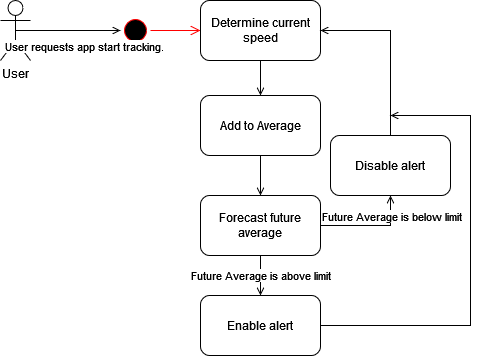
\includegraphics{UserStartedFlow.png}}
\end{figure}

The main automation is effectively a separate loop that invokes the original flow, by checking for location of the user and comparing to a dataset of average speed zones; and similarly the original flow must now return to the invocation loop when it determines it has exited a zone. This is displayed in figure \ref{fig:AutoFlow}.
\begin{figure}
    \centering
    \caption{Flow with automation.}
    \label{fig:AutoFlow}
    \scalebox{0.5}{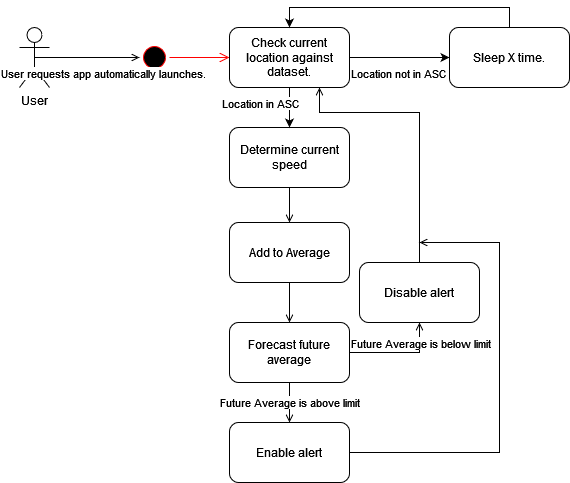
\includegraphics{AutomatedFlow.png}}
\end{figure}

\chapter{Technical Development}
While the actual development of code can be found in appendix \ref{app:GitLog}, it is worthwhile discussing, separately to that, justification and reasoning behind certain decisions and implementations.

\subsection{Settings Page}
Certain parameters of the application are user configurable; for example, except for in Automatic mode, the speed limit can be changed by the user, and the forecast time for the model can be configured by the user. However, the speed limit should be changeable from the main interface of the application, while the forecast time does not need to be. Hence a "settings page" should be created.

\citet{settingsAndroid} provides a guide on how to implement a settings screen, using a \textit{PreferenceScreen} fragment. By using this part of the Android Jetpack library, a developer doesn't have to implement their own Settings system. However, to get to this settings page, the user must interact with something; one idea is for a settings button on the top bar of the application.

\appendix
\chapter{Development Log}\label{app:GitLog}
TestTestTest

\bibliography{finalrep}
\end{document}